\documentclass[journal,twoside,web,onecolumn]{ieeecolor}
\usepackage{generic}
\usepackage{amsmath,amssymb,booktabs,siunitx}
\usepackage[hidelinks]{hyperref}
\usepackage{placeins}
\usepackage{needspace}
\usepackage{caption}
\DeclareCaptionLabelFormat{tabS}{Table~#2}
\DeclareCaptionLabelFormat{figS}{Fig.~#2}
\captionsetup{labelsep=period, font={footnotesize,rm,up}, labelfont={bf,rm,up}, justification=centering}
\captionsetup[table]{labelformat=tabS, position=top, skip=4pt}
\captionsetup[figure]{labelformat=figS, skip=4pt}
\usepackage{graphicx}
\usepackage{tikz}
\usetikzlibrary{positioning,arrows.meta}
\usetikzlibrary{calc}
\renewcommand{\thetable}{S\arabic{table}}
\renewcommand{\thefigure}{S\arabic{figure}}
\renewcommand{\thesection}{S\arabic{section}}
\makeatletter\let\inputtab\@@input\makeatother

\begin{document}
\sloppy
\pagestyle{plain}
\begin{center}
{\large Supplementary Material}\\[3pt]
{\small Segmentation Error and Boundary-Condition Tuning in Computed Coronary FFR: A Controlled In Silico Study}\\[2pt]
{\small Fadillah Yamin, Mohd Azan Mohammed Sapardi, Ming Kwang Tan, Xin Wang, and Mohd-Zulhilmi Ismadi}
\end{center}
\vspace{2pt}

\section{Analysis Pipeline}
Fig.~\ref{fig:pipeline} shows the analysis pipeline. Host vessels were eligible with an image quality of at least 2
(0--4 scale), a taper-fit radius $r_\mathrm{fit}$ of at least 1.0~mm at the lesion center and native narrowing below
40\% DS. The measurement point 20~mm beyond the lesion lay on a vessel of radius at least 0.75~mm, and the FFR before
insertion was at least 0.90.
\begin{figure}[!h]
\centering
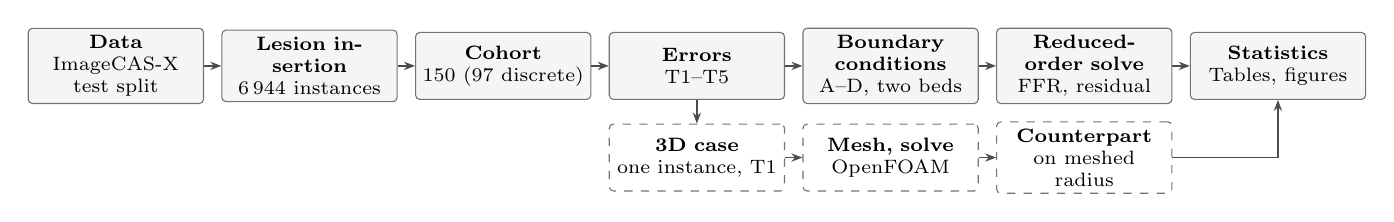
\begin{tikzpicture}[font=\scriptsize,
  box/.style={draw=black!55, fill=black!4, rounded corners=1.5pt, inner sep=2.5pt, align=center, minimum height=8.5mm, text width=2.05cm},
  cfd/.style={box, fill=white, dashed},
  arr/.style={-{Stealth[length=1.4mm]}, draw=black!70, line width=0.5pt}]
\node[box] (d) at (0,0) {\textbf{Data}\\ImageCAS-X test split};
\node[box, right=2.2mm of d] (l) {\textbf{Lesion insertion}\\6\,944 instances};
\node[box, right=2.2mm of l] (c) {\textbf{Cohort}\\150 (97 discrete)};
\node[box, right=2.2mm of c] (e) {\textbf{Errors}\\T1--T5};
\node[box, right=2.2mm of e] (b) {\textbf{Boundary conditions}\\A--D, two beds};
\node[box, right=2.2mm of b] (r) {\textbf{Reduced-order solve}\\FFR, residual};
\node[box, right=2.2mm of r] (st) {\textbf{Statistics}\\Tables, figures};
\node[cfd, below=3mm of e] (x) {\textbf{3D case}\\one instance, T1};
\node[cfd, right=2.2mm of x] (m) {\textbf{Mesh, solve}\\OpenFOAM};
\node[cfd, right=2.2mm of m] (t) {\textbf{Counterpart}\\on meshed radius};
\foreach \u/\v in {d/l, l/c, c/e, e/b, b/r, r/st, x/m, m/t} \draw[arr] (\u) -- (\v);
\draw[arr] (e) -- (x);
\draw[arr] (t.east) -| (st.south);
\end{tikzpicture}
\caption{Analysis pipeline. Shaded boxes: reduced-order arm, run for every instance in one automated run. Dashed
boxes: the 3D case study. Sensitivity analyses and noise floors repeat the reduced-order arm.}\label{fig:pipeline}
\end{figure}

\FloatBarrier
\Needspace{16\baselineskip}
\section{Exclusions}
Table~\ref{tab:excl} lists every exclusion. Protocols C and D require at least two territories that retain a
vessel. A Protocol C fit at its search bound is a failure (two half-voxel throat-error models; 10 of 4\,940
noise-floor draws). Protocol D fits at the $10^{\pm 3}$ bound keep a defined residual and are retained (two missed-branch models, residual 0.08 and 0.11). The bound was also reached by 23 half-voxel and 41 ten-point throat-error models with an increased stenosis, of
which 43 failed the check and 21 passed while materially wrong.
Under Protocol A a vessel break can remove every node with bed outflow (36 discrete, 2 leaky); scored as reclassifications (FFR 1),
these raise the discrete-bed vessel-break reclassification rate from 40\% to 43\%.
\begin{table}[!ht]
\caption{Cells With Excluded Models}\label{tab:excl}
\centering\footnotesize
\begin{tabular}{@{}lllrl@{}}
\toprule
Bed & Error & Protocol & Solved & Excluded (reason: count)\\
\midrule
\inputtab supplement_tables/tab_exclusions_nz.tex 
\bottomrule
\end{tabular}
\end{table}

\FloatBarrier
\Needspace{16\baselineskip}
\section{Mixed-Effects Model of Reclassification}
\begin{table}[!ht]
\caption{Bayesian Logistic Model of Reclassification: Posterior Mean Log-Odds (95\% Interval)}\label{tab:glmm}
\centering\footnotesize
\begin{tabular}{@{}lcc@{}}
\toprule
Term & Discrete bed & Leaky bed\\
\midrule
\inputtab supplement_tables/tab_glmm.tex 
\bottomrule
\end{tabular}
\\[3pt]
\parbox{0.85\textwidth}{\footnotesize Reference levels: T1 (missed branch) and Protocol A. Baseline-band terms are
omitted from the table. Random intercepts for patient and lesion slot. The model agrees with the paired tests in direction. Fitted by variational inference; intervals are
posterior mean $\pm 1.96$ posterior standard deviations from the variational approximation.}
\end{table}

\FloatBarrier
\Needspace{16\baselineskip}
\section{Sensitivity Analyses}
\subsection{Perfusion-Check Threshold}
Table~\ref{tab:thr} gives passes-and-wrong for the topological errors at the 10\% threshold and at the 13\% and 16\% sensitivities.
\begin{table}[!ht]
\caption{Proportion of Models That Pass the Perfusion Check and Are Materially Wrong, \% (Wilson 95\% Interval), by
Perfusion-Check Threshold}\label{tab:thr}
\centering\footnotesize
\begin{tabular}{@{}lllrcccrc@{}}
\toprule
 & & & & \multicolumn{3}{c}{Passes and wrong, \% of $n$} & \multicolumn{2}{c}{At 10\%}\\
\cmidrule(lr){5-7}\cmidrule(l){8-9}
Bed & Errors & Protocol & $n$ & 10\% & 13\% & 16\% & Pass & Wrong among passing, \%\\
\midrule
\inputtab supplement_tables/tab_thresholds.tex 
\bottomrule
\end{tabular}
\\[3pt]
\parbox{0.85\textwidth}{\footnotesize Materially wrong: $|\Delta\mathrm{FFR}| > 0.05$. The 13\% and 16\% thresholds were analyzed as sensitivities. $n$ counts models with a
defined perfusion residual: T2 under Protocols A and B in the leaky bed, $n = 100$; T2 under Protocol B in the
discrete bed, $n = 60$. Protocol D matches every territory flow in all but two models, so its passes-and-wrong and wrong proportions differ by at most one model.}
\end{table}

\FloatBarrier
\Needspace{16\baselineskip}
\subsection{Hyperemic Demand}\label{sec:demand}
With $k = 562$~s$^{-1}$, a vessel with the normal proximal LAD diameter of 3.7~mm carries 214~mL/min, within one standard deviation of the hyperemic flow measured in that artery by continuous thermodilution ($228 \pm 71$ to $293 \pm 102$~mL/min). The cohort's median demand was 2.28~mL/s (137~mL/min) per tree.
The demand constant $k$ was scaled by 0.7 and 1.3 with the same cohort (Table~\ref{tab:demand}). The ordering of
topological against caliber errors, and of Protocols B and C against Protocol A, was unchanged in both beds; the
magnitudes changed because demand moves the clean FFR (leaky-bed median 0.869, 0.801 and 0.741). Tuned topological
passes-and-wrong fell to 3\% (leaky bed, 0.7 times the demand) and stayed at 12--25\% (discrete bed).
\begin{table}[!h]
\caption{Sensitivity to Hyperemic Demand}\label{tab:demand}
\centering\small
\begin{tabular}{@{}llcccccc@{}}
\toprule
Bed & Demand scale & \multicolumn{2}{c}{Flip, \% (Protocol A)} & \multicolumn{2}{c}{Topological flip, \%} &
Passes and wrong, \% & Missed-branch $\Delta$FFR\\
\cmidrule(lr){3-4}\cmidrule(lr){5-6}
 & & Topological & Caliber & B & C & (C, topological) & median, A / C\\
\midrule
Discrete & 0.7 & 32 (25--40) & 6 (3--10) & 12 (8--18) & 18 (12--27) & 12 (7--19) & 0.070 / 0.057 \\
 & 1.0 & 33 (26--41) & 10 (7--15) & 14 (10--20) & 19 (13--28) & 19 (13--28) & 0.095 / 0.077 \\
 & 1.3 & 40 (32--48) & 5 (2--9) & 16 (11--22) & 19 (13--28) & 25 (18--34) & 0.106 / 0.091 \\
Leaky & 0.7 & 20 (16--26) & 6 (4--9) & 7 (4--10) & 9 (5--14) & 3 (1--7) & 0.032 / 0.010 \\
 & 1.0 & 32 (26--38) & 6 (4--9) & 5 (3--8) & 8 (5--13) & 8 (5--13) & 0.047 / 0.015 \\
 & 1.3 & 37 (32--43) & 4 (2--7) & 5 (3--9) & 8 (4--13) & 12 (8--18) & 0.057 / 0.021 \\
\bottomrule
\end{tabular}
\\[3pt]
\parbox{0.9\textwidth}{\footnotesize Demand scale 1.0 is the primary analysis ($k = 562$~s$^{-1}$). Percentages with Wilson 95\%
intervals in parentheses. Missed-branch $\Delta$FFR is over the instances in which Protocol C was defined.}
\end{table}


\FloatBarrier
\Needspace{16\baselineskip}
\subsection{Demand Replication With Re-Selected Cohorts}\label{sec:replication}
The whole pipeline was repeated with $k$ doubled and tripled, with cohorts reselected at that demand. At three times
the demand only 17 instances met the discrete-bed criteria, so the discrete arm is reported at twice the demand
(Table~\ref{tab:repl}). The excess of tuned over re-derived passes-and-wrong at twice the demand was significant in
three of four caliber comparisons and in no topological one.
\begin{table}[!ht]
\caption{Demand Replication: Reclassification and Passes-and-Wrong Rates, \% (Wilson 95\% Interval)}\label{tab:repl}
\centering\footnotesize\setlength{\tabcolsep}{3pt}
\begin{tabular}{@{}lrrcccccccccc@{}}
\toprule
 & & & \multicolumn{2}{c}{Reclass., A} & \multicolumn{2}{c}{Topological reclass.} & \multicolumn{3}{c}{Topological passes and wrong} & \multicolumn{3}{c}{Caliber passes and wrong}\\
\cmidrule(lr){4-5}\cmidrule(lr){6-7}\cmidrule(lr){8-10}\cmidrule(l){11-13}
Bed & $k$ scale & Inst. & Topol. & Caliber & C & D & B & C & D & B & C & D\\
\midrule
\inputtab supplement_tables/tab_replication.tex 
\bottomrule
\end{tabular}
\\[3pt]
\parbox{0.95\textwidth}{\footnotesize Scale 1 is the primary analysis ($k = 562$~s$^{-1}$, primary cohort). Scales 2 and 3 use
cohorts reselected at that demand. Passes and wrong: perfusion residual below 10\% and $|\Delta\mathrm{FFR}| > 0.05$;
denominators are models with a defined residual, as in Table I of the main text.}
\end{table}

\FloatBarrier
\Needspace{16\baselineskip}
\subsection{Grey Zone}\label{sec:grey}
Beyond-zone reclassifications end outside 0.75--0.85 (Table~\ref{tab:grey}); 30\% (discrete) and 33\% (leaky) of clean models lie within.
\begin{table}[!ht]
\caption{Reclassification, Overall and Beyond the Grey Zone (0.75--0.85), \% of Models (Wilson 95\% Interval)}\label{tab:grey}
\centering\footnotesize
\begin{tabular}{@{}llrccrcc@{}}
\toprule
 & & \multicolumn{3}{c}{Topological errors} & \multicolumn{3}{c}{Caliber errors}\\
\cmidrule(lr){3-5}\cmidrule(l){6-8}
Bed & Protocol & $n$ & Reclass. & Beyond zone & $n$ & Reclass. & Beyond zone\\
\midrule
\inputtab supplement_tables/tab_greyzone.tex 
\bottomrule
\end{tabular}
\end{table}

\FloatBarrier
\Needspace{16\baselineskip}
\section{Caliber Error at the Stenosis Throat}\label{sec:throat}
The throat error (T5) re-inserts each lesion with its throat diameter changed by half the in-plane voxel size
(spacing median 0.352~mm; throat radius $\pm 0.088$~mm; 7.3 points of DS, 4.5--9.8) or its DS changed by $\pm 10$ points. The $\pm 10$-point magnitude lies within the published CT-versus-invasive disagreement (standard deviation 12.3--12.4 points). Protocol B equals
Protocol A for this error by construction (Table~\ref{tab:throat}). Protocol C fits at the search bound were excluded
(2 at half a voxel, 8 at $\pm 10$ points). The 64 Protocol D fits at the parameter bound, all with an increased
stenosis, were retained; excluding them would raise passes-and-wrong by up to 13 points.
\begin{table}[!ht]
\caption{Throat Caliber Error: Reclassification and Passes-and-Wrong, \% of Models (Wilson 95\% Interval)}\label{tab:throat}
\centering\footnotesize\setlength{\tabcolsep}{3pt}
\begin{tabular}{@{}llrccc rccc@{}}
\toprule
 & & \multicolumn{4}{c}{Discrete bed (97 instances)} & \multicolumn{4}{c}{Leaky bed (150 instances)}\\
\cmidrule(lr){3-6}\cmidrule(l){7-10}
Error & Protocol & $n$ & Reclass. & Passes and wrong & Beyond zone & $n$ & Reclass. & Passes and wrong & Beyond zone\\
\midrule
$\pm\tfrac12$ voxel pooled & A, B & 194 & 30 (24--37) & 29 (23--36) & 14 (10--20) & 300 & 36 (31--42) & 42 (37--48) & 21 (16--26) \\
 & C & 193 & 38 (31--45) & 57 (50--64) & 22 (17--28) & 299 & 37 (32--43) & 69 (63--74) & 29 (25--35) \\
 & D & 194 & 40 (33--47) & 80 (74--85) & 26 (21--33) & 300 & 38 (33--44) & 81 (76--85) & 29 (24--34) \\
\addlinespace[2pt]
DS $\pm10$ pooled & A, B & 194 & 40 (33--47) & 20 (15--26) & 27 (22--34) & 300 & 42 (37--48) & 40 (34--45) & 35 (30--40) \\
 & C & 187 & 44 (37--52) & 51 (44--58) & 37 (30--44) & 299 & 43 (38--49) & 62 (56--67) & 41 (35--46) \\
 & D & 194 & 45 (38--52) & 75 (68--80) & 40 (34--47) & 300 & 44 (38--49) & 86 (81--89) & 40 (35--46) \\
$\pm\tfrac12$ voxel, $k\times2$ & A, B & 94 & 27 (19--36) & 35 (26--45) & 12 (7--20) & 300 & 29 (24--35) & 44 (39--50) & 12 (9--16) \\
 & C & 94 & 31 (22--41) & 52 (42--62) & 13 (7--21) & 300 & 35 (30--40) & 69 (64--74) & 17 (13--21) \\
 & D & 94 & 34 (25--44) & 73 (64--81) & 18 (12--27) & 300 & 35 (30--41) & 75 (70--80) & 18 (14--22) \\
\addlinespace[2pt]
$\pm\tfrac12$ voxel, $k\times3$ & A, B & -- & -- & -- & -- & 300 & 29 (24--34) & 48 (43--54) & 9 (6--13) \\
 & C & -- & -- & -- & -- & 300 & 34 (29--40) & 68 (62--73) & 15 (12--20) \\
 & D & -- & -- & -- & -- & 300 & 33 (28--39) & 72 (67--77) & 14 (10--18) \\
\bottomrule
\end{tabular}
\\[3pt]
\parbox{0.95\textwidth}{\footnotesize $\pm\tfrac12$ voxel: throat diameter narrowed or widened by half the in-plane voxel size, both signs pooled. DS $\pm10$: diameter stenosis raised or lowered by 10 points, both signs pooled. Passes and wrong: perfusion residual below 10\% and $|\Delta\mathrm{FFR}| > 0.05$. Beyond zone: reclassifications whose corrupted FFR lies outside 0.75--0.85. Protocols A and B coincide for throat errors. Protocol C fits on the search bound are excluded, which reduces $n$. $k\times2$, $k\times3$: demand constant doubled or tripled with the cohort reselected at that demand. Discrete bed: 47 instances at $k\times2$, not analyzed at $k\times3$. Topological reclassification under Protocol A was 50\% (38--62\%) and 34\% (29--40\%) at $k\times2$ and 33\% (28--39\%) at $k\times3$, against 33\% (26--41\%) and 32\% (26--38\%) at the primary demand, where caliber errors away from the throat gave 10\% (7--15\%) and 6\% (4--9\%).}
\end{table}

\FloatBarrier
\Needspace{16\baselineskip}
\section{Territory Granularity}\label{sec:granularity}
Protocols C and D were repeated with each main-branch territory divided again at its first bifurcation (median four territories, discrete; five, leaky). A territory without a surviving vessel entered the residual as a 100\% mismatch; without this rule, discrete topological passes-and-wrong would have risen to 26\%. With the main-branch partition the
procedure reproduced the original results exactly (Table~\ref{tab:gran}). Throat-error models removed from the count
all failed the finer check; none had its FFR corrected, and 76--88\% of tuned throat-error models that passed remained
materially wrong. Reclassifications changed by at most five per cell. The simulated noise floor was computed at
main-branch level only.
\begin{table}[!ht]
\caption{Passes and Wrong, \% (Wilson 95\% Interval), at Main-Branch and Finer Territory Level}\label{tab:gran}
\centering\footnotesize
\begin{tabular}{@{}lllrccc@{}}
\toprule
Bed & Errors & Protocol & $n$ & Main branch & Finer & $p$\\
\midrule
Discrete & T1+T2 & C & 104 & 19 (13--28) & 7 (3--13) & $<0.001$ \\
 & & D & 104 & 20 (14--29) & 3 (1--8) & $<0.001$ \\
 & T3+T4 & C & 194 & 5 (2--9) & 5 (3--9) & 1.0 \\
 & & D & 194 & 18 (13--24) & 23 (18--30) & 0.002 \\
 & T5, $\pm\tfrac12$ voxel & A, B & 194 & 29 (23--36) & 25 (20--32) & 0.016 \\
 & & C & 193 & 57 (50--64) & 51 (44--58) & 0.003 \\
 & & D & 194 & 80 (74--85) & 78 (71--83) & 0.12 \\
\addlinespace[2pt]
Leaky & T1+T2 & C & 171 & 8 (5--13) & 5 (2--9) & 0.07 \\
 & & D & 171 & 5 (3--10) & 2 (1--6) & 0.18 \\
 & T3+T4 & C & 300 & 12 (9--17) & 12 (9--17) & 1.0 \\
 & & D & 300 & 4 (2--7) & 9 (7--13) & $<0.001$ \\
 & T5, $\pm\tfrac12$ voxel & A, B & 300 & 42 (37--48) & 35 (30--41) & $<0.001$ \\
 & & C & 299 & 69 (63--74) & 60 (55--66) & $<0.001$ \\
 & & D & 300 & 81 (76--85) & 81 (76--85) & 1.0 \\
\bottomrule
\end{tabular}
\\[3pt]
\parbox{0.85\textwidth}{\footnotesize Passes and wrong: perfusion residual below 10\% and $|\Delta\mathrm{FFR}| > 0.05$. Main branch: subtrees below each child of the first bifurcation (two or three per tree). Finer: each divided again at its own first bifurcation (median four, discrete; five, leaky). $n$ counts models with a defined residual at both levels; Protocol C fits on the search bound at either level are excluded. For throat errors the FFR of Protocols A and B is the same at both levels and only the residual changes. $p$: exact McNemar test, paired by model.}
\end{table}

\FloatBarrier
\Needspace{16\baselineskip}
\section{Overlap and Topology of the Corrupted Trees}\label{sec:overlap}
Each tree was represented as cylinders of node radius and element length (a tube model) and compared with its clean
tree; no error changed the number of connected components (Table~\ref{tab:overlap}). Among the topological errors that changed the decision, 91\% (79--96\%, discrete) and 62\% (51--72\%, leaky) kept a whole-scan DSC at or above the
inter-observer 0.928. The AUC of tree DSC for a Protocol A reclassification was 0.65 (discrete) and 0.79 (leaky) overall
and 0.54 and 0.70 within topological errors. The taper DSC exceeds 0.928 because it narrows only the tree beyond
the lesion (about 40\% of its volume).
\begin{table}[!ht]
\caption{Tube-Model Overlap of Corrupted Trees, Median (IQR), and Protocol A Decision Changes}\label{tab:overlap}
\centering\footnotesize
\begin{tabular}{@{}llrcccrc@{}}
\toprule
Bed & Error & $n$ & DSC, tree & DSC, scan & clDice & Flow lost, \% & Reclass. A, \% \\
\midrule
Discrete & T1 & 77 & 0.975 (0.947--0.984) & 0.985 (0.977--0.991) & 0.940 (0.903--0.963) & 27 (14--43) & 27 (19--38) \\
 & T2 & 96 & 0.893 (0.701--0.937) & 0.935 (0.888--0.960) & 0.847 (0.544--0.907) & 30 (15--100) & 40 (29--53)$^a$ \\
 & T3 & 97 & 0.996 (0.995--0.997) & 0.998 (0.998--0.998) & 1.000 & 0 & 7 (4--14) \\
 & T4 & 97 & 0.971 (0.947--0.981) & 0.983 (0.974--0.989) & 1.000 & 0 & 13 (8--22) \\
Leaky & T1 & 118 & 0.969 (0.946--0.980) & 0.983 (0.975--0.990) & 0.930 (0.899--0.957) & 9 (6--17) & 18 (12--26) \\
 & T2 & 149 & 0.895 (0.721--0.936) & 0.934 (0.886--0.962) & 0.855 (0.517--0.899) & 14 (7--56) & 43 (35--51) \\
 & T3 & 150 & 0.997 (0.995--0.998) & 0.998 (0.998--0.999) & 1.000 & 0 & 2 (1--6) \\
 & T4 & 150 & 0.972 (0.951--0.981) & 0.983 (0.976--0.988) & 1.000 & 0 & 9 (6--15) \\
\midrule
\multicolumn{3}{@{}l}{T2, right coronary artery} & 0.62--0.63 & 0.85--0.86 & 0.45--0.49 & & \\
\bottomrule
\end{tabular}
\\[3pt]
\parbox{0.85\textwidth}{\footnotesize Reclass. A: under Protocol A, Wilson 95\% interval. Flow lost: share of the clean model's bed outflow on deleted nodes. $^a$ $n = 60$; right coronary breaks leave no discrete outlet under Protocol A.}
\end{table}

\FloatBarrier
\Needspace{16\baselineskip}
\section{Detection Before and During Tuning}\label{sec:detector}
Positives are error models; negatives are the correct-anatomy draws of the simulated floor before tuning. Correct anatomy without noise has a residual below $10^{-8}$; with noise its median is 0.10, and 48\% (discrete) and 50\% (leaky) of draws exceed the 10\% check. With noise-free targets the pre-tuning residual of topological errors gave an AUC of 0.77 (0.71--0.82, discrete) and 0.22 (0.18--0.27, leaky) and flagged 83\% and 19\% at the 10\% check. With the error models' targets carrying the same noise (Table~\ref{tab:matched}), the AUC was 0.82 (discrete) and 0.56 (leaky).

\FloatBarrier
\Needspace{16\baselineskip}
\section{Noise Floors}\label{sec:floor}
The perfusion-check bound is $1.96 \times (10\text{--}15\%) \approx 20$--29\% for one model output against one
measurement, from the within-subject variation of hyperemic myocardial blood flow. The simulated floor perturbs,
in 20 draws per instance, cardiac output (relative standard deviation 0.05), aortic pressure (0.056), viscosity (0.02),
territory flow shares (0.10) and the measured territory flows (0.083). Tuned as in Protocol C, correct anatomy was reclassified in 6.2\% (discrete) and 7.2\% (leaky) of draws (median $|\Delta$FFR$|$ 0.012, 95th percentile 0.05) and passed the check in 72\%.
Table~\ref{tab:matched} tunes every error model to the floor's noisy targets and adds a Protocol D floor. Rates are means over 20 draws per instance with patient-level cluster-bootstrap intervals; the excess is the per-draw difference from the correct-anatomy model of the same instance, bed and draw, and $n$ counts models with a defined residual.
\begin{table}[!ht]
\caption{Passes and Wrong, \% of Models, With Error Models and Correct Anatomy Tuned to the Same Noisy Targets (Noise-Free: Table I)}\label{tab:matched}
\centering\footnotesize\setlength{\tabcolsep}{4pt}
\begin{tabular}{@{}llrrccrrcc@{}}
\toprule
 & & \multicolumn{4}{c}{Discrete bed} & \multicolumn{4}{c}{Leaky bed}\\
\cmidrule(lr){3-6}\cmidrule(l){7-10}
Error & Protocol & $n$ & Noise-free & Matched & Excess over floor & $n$ & Noise-free & Matched & Excess over floor\\
\midrule
\inputtab supplement_tables/tab_noise_matched.tex 
\bottomrule
\end{tabular}
\end{table}

\FloatBarrier
\Needspace{3\baselineskip}
\section{Three-Dimensional Case Study: Mesh Checks}\label{sec:cfd}
Surfaces were extracted by marching cubes with Taubin smoothing; meshes of 3.5--3.9 million cells (cfMesh) had
25~\textmu m cells within $\pm 4$~mm of the throat and four boundary layers. OpenFOAM simpleFoam (ESI v2406; SIMPLE;
bounded second-order upwind) ran 3\,000 iterations per solve to scaled residuals below $10^{-5}$. A finer throat zone (12.5~\textmu m, 6.24 and 8.31 million cells) raised the baseline FFR from 0.8698 to 0.8716 and 0.8718
(0.0019--0.0021). Outlet flows changed by at most 0.25\%, above the idealized-case discretization uncertainty of $5.5\times10^{-4}$,
so the patient-case uncertainty is about 0.002, against an error effect of 0.074. The finest mesh missed the strict residual limit (velocity residual $1.08\times10^{-5}$) with a steady inlet pressure. The lesion carried about 10~mL/min (tree inflow 0.68~mL/s in 3D, 0.65--0.67~mL/s in the cohort model). At the meshed throat radius of 0.276~mm the mean velocity is about 0.7~m/s and the Reynolds number about 110, within the laminar regime.


\end{document}
